\section{Test effettuati} %TODO Graziano, Federica, Carlo i test effettuati da voi
In questa sezione si elencano i test effettuati per ogni prodotto di progetto.
Per i test di accessibilità eseguiti in remoto, il sito è stato caricato su
GitHub Pages.

\subsection{Validazione XHTML}
Ogni pagina è stata validata con il tool offerto da W3C all'indirizzo
\texttt{http://validator.w3.org/\#validate\_by\_input}.

\subsection{Validazione CSS}
Ogni foglio di stile CSS è stato validato con il tool offerto da W3C
all'indirizzo
\texttt{https://jigsaw.w3.org/css-validator/\#validate\_by\_input}.

\subsection{Validazione XML e XSD}
Il file XML dove sono salvati i commenti è stato validato rispetto al suo
schema XSD con il tool offerto da \textit{freeformatter.com} all'indirizzo
\texttt{http://www.freeformatter.com/xml-validator-xsd.html}.

\subsection{Validazione XSLT}
Il file XSLT che permette di trasformare il file XML dove sono salvati i
commenti è stato validato (si è anche verificato il suo corretto
funzionamento) con il tool offerto da \textit{freeformatter.com} all'indirizzo
\texttt{http://www.freeformatter.com/xsl-transformer.html}.

\subsection{JavaScript}
Ogni script JavaScript è stato analizzato tramite il tool di analisi statica di
\textit{WebStorm}, affinchè venissero trovati errori e miglioramenti al codice.

Ogni frammento di codice è stato testato in locale ed in remoto non tralasciando alcun valore nel dominio dei possibili valori in ingresso. Ogni
test è stato effettuato tenendo visibile la \textbf{Javascript Console} del
browser, così da notare eventuali warning o errori nel codice. I test hanno
avuto esito positivo sul prodotto finale.

\subsection{Perl e CGI}
Ciascuno degli script Perl e CGI è stato verificato in locale, con esiti
positivi.

\subsection{Cynthia Says}
Uno dei tool che è stato utilizzato per l'accessibilità delle pagine è Cynthia
Says, inserendo l'URL di ogni pagina caricata su GitHub Pages e richiedendo la
conformità a WCAG 2.0 AAA. Questa scelta è dovuta al fatto che i tentativi per
verificare l'accessibilità di una pagina sono limitati a 10 nell'arco di 24
ore.
Di seguito vengono riportati i risultati ottenuti per \textbf{tutte} le pagine
del sito:

\begin{table}[h!]
\begin{center}
\begin{tabular}{ | l | c | }
  \hline
  Conformità & Esito \\
  \hline
  WCAG 2.0 A & Conforme \\
  \hline
  WCAG 2.0 AA & Conforme \\
  \hline
  WCAG 2.0 AAA & Non conforme \\
  \hline
\end{tabular}
\caption{Conformità allo standard WAI 2.0 X WCAG}
\end{center}
\end{table}

Le pagine del sito non sono conformi a WCAG 2.0 AAA poichè:
\begin{enumerate}
\item \textit{Cynthia Says} non riconosceva come pagine di aiuto ``Mappa del
sito" e ``F.A.Q.";
\item il contrasto richiesto per il terzo grado di accessibilità era troppo
elevato per poter garantire una resa grafica piacevole del sito.
\end{enumerate}

\subsection{WAVE}
WAVE (Web Accessibility Evaluation Tool) è uno strumento offerto da
\textit{WebAIM} (WEB Accessibility In Mind) per verificare l'accessibilità
delle pagine. Questo strumento analizza una pagina e fornisce errori,
avvertimenti (warnings), caratteristiche positive, struttura basilare di una
pagina e indicazioni sul contrasto.

Più in particolare, sono stati corretti gli errori trovati (relativi agli
standard 508 e WCAG) non relativi alla lingua delle pagine, dal momento che
nonostante il tag html fosse ben-formato e contenente l'indicazione sulla
lingua utilizzata nella pagina in modo corretto, il sito continuava a
segnalare il falso positivo.

I warnings sono stati corretti solo se effettivamente utili; questo dal
momento che sono stati introdotti volutamente titoli o link ridondanti per
aiutare l'utente a capire dove si trova e che l'uso dei tabindex viene
segnalato come warning, anche se questi sono stati messi per permettere
all'utente di raggiungere subito i link della pagina più rilevanti, saltando
elementi di navigazione o breadcrumb a seconda dei casi.

I contrasti dei colori sono stati regolati per riuscire a superare almeno il
livello di accessibilità WCAG 2.0 AA.

\subsection{Vischeck}
Vischek è uno strumento che permette di visualizzare immagini e pagine web
come le vedrebbe una persona che presenta deficit visivi quali:
\begin{itemize}
\item Deuteranope: una forma di deficit di colore rosso/verde
\item Protanope: un'altra forma di deficit di colore rosso/verde
\item Tritanope: una forma di parziale o insufficiente discriminativa per il blu e il violetto
\end{itemize}
A causa del fatto che lo strumento per analizzare le pagine web era momentaneamente inutilizzabile sono state effettuate delle prove attraverso degli screen delle pagine web
valutando la visione generale che avrebbero avuto utenti affetti dai deficit precedentemente
esposti.

\begin{figure}[H]
\begin{minipage}{0.45\textwidth}
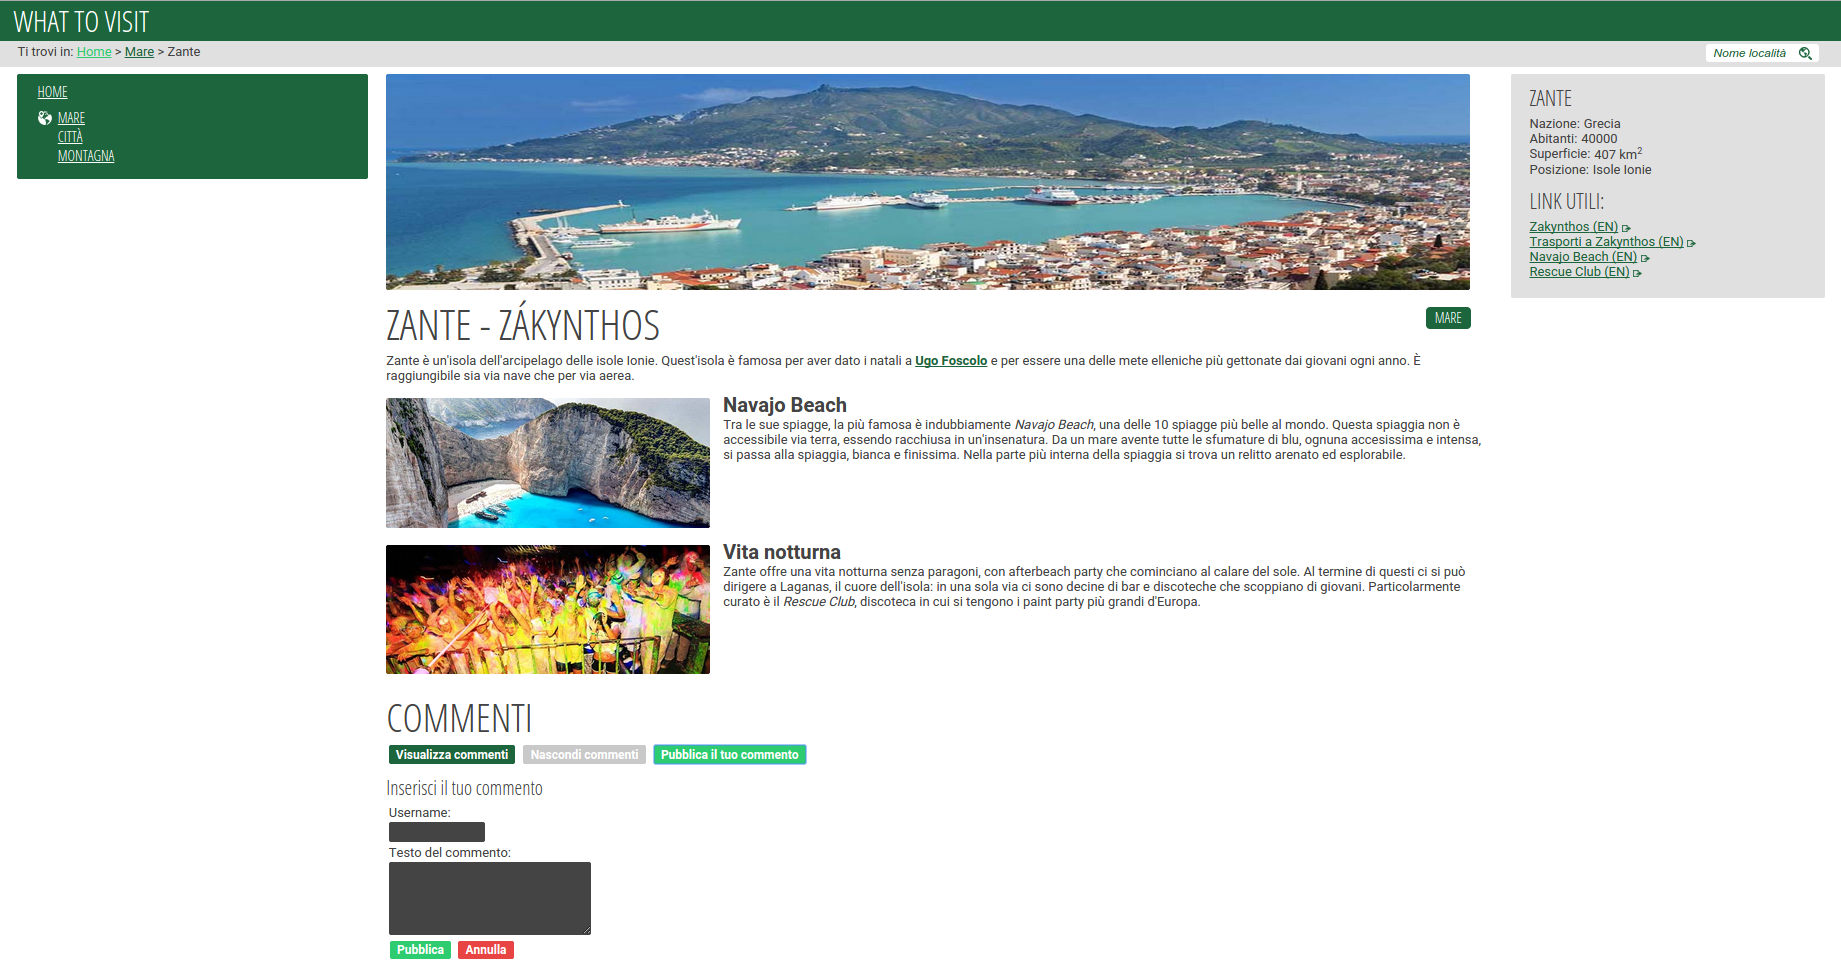
\includegraphics[width=\linewidth]{images/screen/zante.png}
\subcaption{Pagina originale (nessun deficit visivo presente)}
\end{minipage}
\hspace{\fill}
\begin{minipage}{0.45\textwidth}
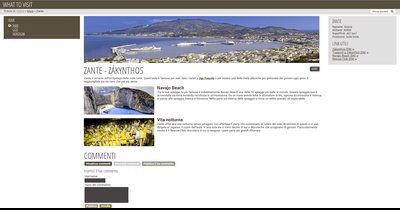
\includegraphics[width=\linewidth]{images/screen/deuteranope.jpg}
\subcaption{Deuteranope}
\end{minipage}
\vspace*{0.5cm}
\begin{minipage}{0.45\textwidth}
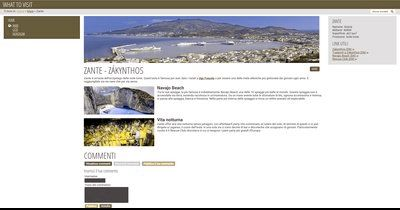
\includegraphics[width=\linewidth]{images/screen/protanope.jpg}
\subcaption{Protanope}
\end{minipage}
\hspace{\fill}
\begin{minipage}{0.45\textwidth}
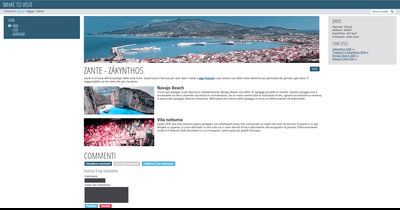
\includegraphics[width=\linewidth]{images/screen/tritanope.jpg}
\subcaption{Tritanope}
\end{minipage}
\caption{Test con Vischek su una pagina di una località}\label{multiavp}
\end{figure}

Dalle quattro immagini si può vedere come le pagine rimangano comunque accessibili e
in particolare i link sono comunque visibili e ben distinguibili dall'utente.

\subsection{Fangs}\label{sec:fangs}
\textit{Fangs} è un'estensione per i browser che consente di visualizzare un
sito nello stesso modo in cui verrebbe visualizzato da uno screen reader,
fornendo il testo come sarebbe letto da questo dispositivo, la lista delle
intestazioni e la lista dei link presenti nella pagina.

Sono state controllate tutte le pagine, con esito positivo: le intestazioni
seguono l'ordine logico pensato dai componenti del gruppo, i link sono
visualizzati nell'ordine aspettato e non sono presenti elementi estranei nel
testo corrispondente all'audio che sentirebbe un utente con screen reader,
mentre gli aiuti come il ``salta la navigazione" sono presenti.

\subsection{Lynx}\label{sec:lynx}
Le pagine del sito sono state anche navigate tramite il browser testuale
\texttt{lynx}, affinchè si potesse verificare la facilità d'uso di
\textit{What To Visit} anche per gli utenti che fanno uso di questo
strumento di navigazione.

\subsection{Compatibilità con i vari Browser}
In sito \textit{What To Visit} è stato testato su vari browser e su
diverse versioni di questi (sia desktop che mobile). 
In particolare risulta compatibile in tutte le sue funzionalità, 
eccetto la geolocalizzazione e la visualizzazione dei commenti
degli utenti, con i seguenti in versione desktop:
\begin{itemize}
\item \textbf{Google Chrome:} versione 40.0+ 
\item \textbf{Mozilla Firefox:} versione 32.0.3+
\item \textbf{Internet Explorer:} versioni 9+
\item \textbf{Opera:} versione 12.16+
\item \textbf{Safari:} versione 5.0+
\item \textbf{Maxthon:} versione 0.9.0.31+ (per Linux)
\end{itemize}

Inoltre, in versione mobile su:
\begin{itemize}
\item \textbf{Google Chrome:} versione 40.0+ 
\item \textbf{Mozilla Firefox:} versione 35+  
\end{itemize}

\subsubsection{Internet Explorer}
Per testare il sito sulle varie versioni di Internet Explorer è stato utilizzato lo strumento
\textit{IETester} disponibile gratuitamente online. Attraverso questo è stato rilevato che, fino alla versione 8 compresa del browser, gli script che si occupano di visualizzare i commenti e di rendere cliccabili le immagini delle categotrie in home non funzionano.

\subsubsection{Geolocalizzazione}
La funzionalità di geolocalizzazione offerta da \textit{What To Visit} è stata
testata con tutti i browser precedentemente elencati tuttavia non risulta compatibile,
in quanto non supportata, da Internet Explorer 8 (e versioni precedenti) e Maxthon per Linux (le altre versioni di Maxthon non sono state provate).

\subsubsection{Visualizzazione commenti degli utenti}
Nel sito è prevista la visualizzazione, per ogni località, dei commenti inseriti dagli utenti.
Tale funzionalità tuttavia è supportata in tutti i browser testati ad eccezione di Internet Explorer, come spiegato nella sezione \ref{sec:visComm}.
